\documentclass[11pt,a4paper]{article}

\usepackage[utf8]{inputenc}
\usepackage[T1]{fontenc}
\usepackage[spanish]{babel}
\usepackage{amsmath,amssymb,amsthm}
\usepackage{graphicx}
\usepackage{hyperref}
\usepackage{enumitem}
\usepackage{booktabs}
\usepackage{listings}
\usepackage{xcolor}
\usepackage{geometry}
\usepackage{float}
\usepackage{mathtools}
\usepackage{algorithm}
\usepackage{algpseudocode}
\usepackage{titlesec}
\usepackage[numbers]{natbib}

\algrenewcommand\algorithmicrequire{\textbf{Requiere}}
\algrenewcommand\algorithmicensure{\textbf{Garantiza}}
\algrenewcommand\algorithmicend{\textbf{fin}}
\algrenewcommand\algorithmicfor{\textbf{para}}
\algrenewcommand\algorithmicdo{\textbf{hacer}}
\algrenewcommand\algorithmicif{\textbf{si}}
\algrenewcommand\algorithmicthen{\textbf{entonces}}
\algrenewcommand\algorithmicelse{\textbf{si no}}
\algrenewcommand\algorithmicwhile{\textbf{mientras}}
\algrenewcommand\algorithmicrepeat{\textbf{repetir}}
\algrenewcommand\algorithmicuntil{\textbf{hasta}}
\algrenewcommand\algorithmicreturn{\textbf{devolver}}

\geometry{margin=2.5cm}
\setlength{\parindent}{0pt}
\setlength{\parskip}{0.5em}
\titleformat{\section}{\normalfont\Large\bfseries}{\thesection}{1em}{}
\titleformat{\subsection}{\normalfont\large\bfseries}{\thesubsection}{1em}{}

\hypersetup{
    colorlinks=true,
    linkcolor=blue,
    urlcolor=blue,
    citecolor=blue
}

\begin{document}

\begin{center}
    \vspace*{-1cm}
    {\LARGE \textbf{Instituto Politécnico Nacional}}\par
    \vspace{0.5em}
    {\Large \textbf{Escuela Superior de Cómputo}}\par
    \vspace{0.5em}
    {\Large \textbf{Ingeniería en Inteligencia Artificial}}\par
    \vspace{0.5em}
    {\Large \textbf{Algoritmos Bioinspirados}}\par
    \vspace{2em}
    {\large \textbf{Sistema de Planificación de Tareas mediante Algoritmos Genéticos}}\par
    \vspace{2em}
    {\large \textbf{Autores:} Gonzalez Pérez Monserrat y Zamudio López Leonardo.}\par
    \vspace{0.4em}
    {\large \textbf{Grupo:} 5BM2}\par
\end{center}

\vspace{1.5em}
\tableofcontents
\clearpage


\begin{abstract}
Este trabajo presenta el marco teórico y técnico de un sistema para la resolución del problema de planificación de tareas mediante algoritmos genéticos. El problema se modela como una instancia del Job Shop Scheduling Problem, donde cada trabajo está compuesto por operaciones con precedencias internas y recursos compartidos. El objetivo del sistema es minimizar el tiempo total de ejecución, medido mediante el makespan, bajo restricciones de precedencia y disponibilidad de máquinas. Para ello, se propone un algoritmo evolutivo que codifica soluciones como permutaciones de operaciones, evalúa su calidad mediante una función objetivo y aplica operadores de selección, cruce y mutación para mejorar iterativamente la población. La arquitectura del sistema está organizada en frontend, backend REST y capa de cómputo asíncrono con Celery, apoyada en MongoDB y Redis. El documento presenta la formalización matemática del problema, la lógica de decodificación de una solución, la estructura del algoritmo genético y el flujo de ejecución del sistema desarrollado.
\end{abstract}

\noindent\textbf{Palabras clave:} optimización combinatoria, planificación de tareas, Job Shop Scheduling, algoritmos genéticos, bioinspiración, makespan, Celery, Flask, React.

\section{Marco teórico de algoritmos bioinspirados}

\subsection{Introducción}

Los algoritmos bioinspirados son métodos computacionales inspirados en procesos naturales, tales como la evolución biológica, el comportamiento de enjambres, la adaptación de sistemas inmunológicos o la dinámica de colonias de insectos. Su objetivo no es reproducir exactamente la biología, sino abstraer principios generales que permitan resolver problemas complejos cuando los métodos clásicos resultan poco prácticos.

Los algoritmos bioinspirados se distinguen por:

\begin{itemize}
    \item explorar espacios de soluciones de alta dimensionalidad;
    \item usar poblaciones de candidatos, no una única solución;
    \item combinar exploración y explotación;
    \item tolerar ruido y no convexidad;
    \item adaptarse mediante iteraciones de mejora.
\end{itemize}

Dentro de esta categoría, los algoritmos genéticos son uno de los paradigmas más representativos, tal como se expone en la formulación clásica de Goldberg y en los tratados de Eiben y Smith sobre computación evolutiva~\cite{goldberg1989genetic,eiben2015introduction}. Asimismo, la referencia de curso de Coello Coello aporta una visión didáctica de la computación evolutiva y del marco conceptual de la optimización bioinspirada~\cite{coello2026introduccion}.

\subsection{Algoritmos genéticos}

Un algoritmo genético (AG) es una técnica de optimización evolutiva que imita la evolución natural por selección, reproducción y variación genética. Se parte de una población inicial de soluciones candidatas, cada una codificada como un cromosoma.

Cada individuo representa una posible solución al problema. El algoritmo asigna a cada individuo una aptitud o fitness, que mide qué tan buena es la solución conforme a la función objetivo. A partir de allí, se aplican operadores evolutivos:

\begin{enumerate}
    \item \textbf{Selección}: elegir individuos con mayor fitness para reproducirse.
    \item \textbf{Cruce}: combinar dos cromosomas para generar descendencia.
    \item \textbf{Mutación}: alterar aleatoriamente parte del cromosoma para introducir diversidad.
    \item \textbf{Reemplazo}: sustituir parte de la población por la nueva generación.
\end{enumerate}

La evolución se repite durante varias generaciones hasta alcanzar un criterio de parada, por ejemplo, un número máximo de iteraciones, convergencia del fitness o tiempo máximo.

\subsubsection{Representación cromosómica}

Una solución se representa por un vector o cadena de genes. En un problema de programación, cada gen puede codificar una operación, una máquina o un orden relativo entre tareas. Un cromosoma puede representar una permutación de operaciones o una asignación de prioridad.

Si un cromosoma es $x = (x_1, x_2, \dots, x_L)$, con $L$ genes, la posición del gen determina el orden de ejecución o la prioridad de una operación en la secuencia.

\subsubsection{Función de adaptación}

Dada una solución $x$, el algoritmo evalúa su calidad mediante una función de fitness $f(x)$ que normalmente se construye a partir de la función objetivo del dominio. En el caso de minimización, suele usarse

$$
F(x) = \frac{1}{1 + f(x)}
$$

para convertir una función objetivo no acotada en un valor proporcional a la calidad. En el problema de programación de tareas, la función objetivo puede ser el makespan:

$$
F(x) = \frac{1}{1 + C_{\max}(x)}.
$$

Esto hace que los individuos con menor makespan tengan mayor fitness.

\subsubsection{Selección}

La selección favorece la reproducción de soluciones mejores. Un método clásico es la selección por torneo. Dados dos o más individuos, se comparan sus fitness y se selecciona el mejor. También existen la ruleta proporcional o la selección por ranking.

La idea es mantener una presión selectiva sin destruir por completo la diversidad. Formalmente, si la población es $P_t$, la selección define una probabilidad de elección

$$
P(i \in P_t) = \frac{F(i)}{\sum_{j \in P_t} F(j)}.
$$

\subsubsection{Cruce}

El cruce combina información genética de dos progenitores para producir descendencia. En problemas de permutación, se usan operadores como:

\begin{itemize}
    \item Order Crossover (OX),
    \item Partially Mapped Crossover (PMX),
    \item Position-Based Crossover,
    \item Cycle Crossover (CX).
\end{itemize}

El objetivo es preservar parcialmente el orden de las operaciones y generar soluciones factibles. Supongamos que dos padres son $p_1 = (a,b,c,d,e)$ y $p_2 = (e,c,a,d,b)$. Un cruce por orden toma una sección de referencia de un progenitor y rellena el resto respetando el orden de aparición del otro progenitor.

\subsubsection{Mutación}

La mutación introduce variabilidad aleatoria para evitar la convergencia prematura. En problemas de permutación, puede consistir en:

\begin{itemize}
    \item intercambio de dos posiciones;
    \item inversión de un bloque;
    \item desplazamiento de un elemento a otra posición.
\end{itemize}

Si $x$ es el cromosoma y $i,j$ dos índices, una operación de intercambio es:

$$
x_i \leftrightarrow x_j.
$$

Con esto se altera parcialmente la estructura del individuo sin perder la representación válida.

\subsubsection{Convergencia y diversidad}

La evolución no solo debe mejorar la calidad promedio, sino también mantener diversidad. Si la población se acerca demasiado rápidamente a una misma solución, el algoritmo puede quedar atrapado en un óptimo local. Por ello, las tasas de mutación, la selección y la estrategia de reemplazo son parámetros críticos.

\subsection{Algoritmos bioinspirados relacionados}

Además de los algoritmos genéticos, existen otros enfoques bioinspirados ampliamente usados en optimización:

\begin{itemize}
    \item \textbf{Optimización por colonia de hormigas (ACO)}: inspira el comportamiento de búsqueda de caminos por parte de las hormigas. Las hormigas depositan feromonas; los caminos con menores costes reciben mayor concentración de feromonas.
    \item \textbf{Optimización por enjambres de partículas (PSO)}: cada partícula mantiene posición y velocidad; la mejor posición personal y la mejor global influyen en la evolución.
    \item \textbf{Algoritmos de enjambre} y \textbf{simulated annealing}: usan analogías con física y comportamiento colectivo.
\end{itemize}

Todos estos enfoques comparten el principio de buscar soluciones aceptables en espacios complejos, sin depender de derivadas o de la estructura convexa del problema.

\section{Fundamentos matemáticos de la evolución artificial}

\subsection{Población, genotipo y fitness}

Un algoritmo genético trabaja con una población de soluciones candidatas, no con una única solución. Sea

$$
P_t = \{x_1^{(t)}, x_2^{(t)}, \dots, x_N^{(t)}\},
$$

la población en la generación $t$, donde cada individuo $x_i^{(t)}$ representa una posible solución del problema. En el contexto de la programación de tareas, cada individuo es un cromosoma que codifica una asignación o una secuencia de prioridad para las operaciones. El valor asociado a cada cromosoma se mide mediante una función de evaluación $f(x_i^{(t)})$, que normalmente corresponde a una medida de costo o penalización.

En la mayoría de los problemas de optimización, el objetivo es minimizar un costo. Por ejemplo, en el problema de scheduling, el costo puede ser el makespan:

$$
f(x) = C_{\max}(x).
$$

Sin embargo, para incorporar la selección natural de forma más conveniente, se define un valor de adaptación o fitness, que transforma la función objetivo en un criterio de preferencia. Una elección clásica es:

$$
F(x) = \frac{1}{1 + f(x)},
$$

cuando se desea minimizar $f(x)$. Esta transformación cumple dos propósitos: hace que los individuos con mejor calidad tengan mayor fitness, y evita dividir entre cero cuando el costo es nulo o muy pequeño.

La evolución artificial puede describirse como una secuencia recursiva de poblaciones:

$$
P_0 \xrightarrow{\text{selección}} P_1 \xrightarrow{\text{cruce y mutación}} P_2 \rightarrow \dots \rightarrow P_T,
$$

donde cada generación se obtiene a partir de la anterior mediante operadores de selección, reproducción y variación. La idea central es que la población no es estática: cada iteración conserva parte de la información útil y agrega diversidad para explorar nuevas soluciones.

\subsection{Selección como presión evolutiva}

La selección es el mecanismo que favorece a los individuos de mejor calidad. Dada una población $P_t$, el algoritmo asigna una probabilidad de supervivencia o reproducción a cada individuo en función de su fitness. En una versión proporcional, la probabilidad de elegir un cromosoma $x_i$ es:

$$
\Pr(x_i \text{ es elegido}) = \frac{F(x_i)}{\sum_{j=1}^{N} F(x_j)}.
$$

La selección introduce una presión evolutiva, porque los individuos con mejor rendimiento tienen más oportunidades de reproducirse, mientras que los peores tienden a desaparecer. Sin embargo, si la presión es excesiva, el algoritmo puede converger prematuramente hacia un buen pero no óptimo local. Por ello, la selección no debe ser ni demasiado débil ni demasiado fuerte.

En la práctica, existen diversos métodos de selección, como la selección por torneo, la ruleta proporcional y la selección por ranking. En este proyecto se usa selección por torneo, donde un conjunto pequeño de individuos compite y se selecciona el mejor de ese subconjunto. Esta estrategia es especialmente útil en problemas combinatorios, porque reduce el costo computacional y mantiene un equilibrio razonable entre explotación y exploración.

\subsection{Cruce como mezcla de material genético}

El operador de cruce combina la información de dos progenitores para producir descendencia. Formalmente, si $x^{(p_1)}$ y $x^{(p_2)}$ son dos cromosomas, el cruce define una operación

$$
\mathcal{C}(x^{(p_1)}, x^{(p_2)}) = (x^{(h_1)}, x^{(h_2)}),
$$

que produce dos hijos con características heredadas de ambos padres. En problemas de permutación o secuenciación, no basta con combinar bits arbitrarios, porque se deben preservar propiedades de factibilidad, como la ausencia de duplicados o la coherencia de precedencias.

Por esta razón, en programación de tareas suelen usarse operadores de cruce especializados, como order crossover (OX), partially mapped crossover (PMX) o variantes de intercambio segmentado. La idea general es conservar fragmentos útiles de un progenitor y completar la información faltante con la estructura del otro padre, manteniendo la viabilidad de la solución.

En términos intuitivos, el cruce hace que la población «aprenda» combinando componentes exitosos de soluciones previas. Si las dos soluciones parentales tienen buena calidad, la recombinación puede producir hijos con mejor rendimiento al combinar rasgos válidos de ambos.

\subsection{Mutación como fuente de diversidad}

La mutación es el operador responsable de introducir variación aleatoria en la población. Su finalidad es evitar que el algoritmo quede atrapado en un óptimo local, especialmente cuando la mayoría de los individuos empiezan a ser muy parecidos entre sí. Si una población pierde diversidad, la selección se vuelve dominante y la exploración desaparece.

En un cromosoma $x = (x_1, x_2, \dots, x_L)$, una mutación puede consistir en intercambiar dos genes, invertir un bloque de genes o alterar una posición con cierta probabilidad. Por ejemplo, una operación de intercambio entre dos posiciones $i$ y $j$ se representa como:

$$
x_i \leftrightarrow x_j.
$$

La mutación no debe aplicarse con demasiada frecuencia, porque entonces el algoritmo se comporta como una búsqueda aleatoria. Pero tampoco debe ser demasiado rara, porque en ese caso la diversidad desaparece y la población converge prematuramente. Por eso se usa una tasa de mutación $p_m$ que controla la intensidad del cambio aleatorio.

\subsection{Diversidad, entropía y convergencia prematura}

La diversidad de una población es un concepto clave para evaluar si el algoritmo sigue explorando soluciones distintas. Una medida simple, aunque no única, es la distancia promedio entre cromosomas:

$$
D(P_t) = \frac{2}{N(N-1)} \sum_{i<j} d(x_i^{(t)}, x_j^{(t)}),
$$

 donde $d(\cdot,\cdot)$ representa una distancia apropiada entre individuos. En problemas de permutación, esta distancia puede interpretarse como la discrepancia entre órdenes de prioridad o la cantidad de diferencias entre posiciones de operaciones.

Cuando $D(P_t)$ baja significativamente, la población tiende a encogerse alrededor de soluciones similares. Este fenómeno se conoce como convergencia prematura. En términos de optimización, puede ser problemático porque el algoritmo deja de explorar y se queda en una región local del espacio de soluciones. Por ello, la combinación entre selección, cruces y mutación debe mantener una diversidad mínima suficiente durante varias generaciones.

La convergencia, por otra parte, es deseable en la medida en que la mejor solución encontrada mejora progresivamente. Se dice que el algoritmo converge cuando la calidad de la población mejora y la mejor solución observada se estabiliza. Formalmente, si $M_t = \min_{x \in P_t} f(x)$, la convergencia se observa cuando $M_t$ deja de disminuir de forma significativa a lo largo de varias generaciones. Sin embargo, la convergencia no garantiza optimalidad global; en la práctica, la meta es encontrar soluciones suficientemente buenas dentro de un presupuesto computacional razonable.

\subsection{Teoría intuitiva de la exploración y la explotación}

La evolución artificial se apoya en un equilibrio entre dos dinámicas complementarias:

\begin{itemize}
    \item \textbf{Exploración}: la capacidad de visitar regiones distintas del espacio de soluciones, principalmente a través de la mutación y de la recombinación de individuos distintos.
    \item \textbf{Explotación}: la capacidad de reforzar soluciones ya prometedoras mediante la selección y la reproducción de individuos con mejor fitness.
\end{itemize}

Si el algoritmo explora demasiado, puede perder rápidamente soluciones prometedoras y requerir más tiempo para encontrar buenas soluciones. Si explota demasiado, corre el riesgo de caer en óptimos locales. La estrategia efectiva es adaptar la presión selectiva y la tasa de mutación para mantener una población equilibrada.

En problemas como el Job Shop Scheduling Problem, esta idea es especialmente relevante, porque el espacio de soluciones es enorme, discreto y altamente no convexo. No existe una trayectoria lineal hacia la solución óptima, y la forma del paisaje de fitness cambia conforme se modifican las asignaciones y los tiempos de procesamiento. Por eso, los algoritmos genéticos resultan adecuados: ofrecen una estrategia robusta para explorar combinaciones complejas sin depender de gradientes ni de convexidad.

\section{Definición del problema}

\subsection{Problema de programación de tareas}

El problema de planificación de tareas puede interpretarse como una instancia del Job Shop Scheduling Problem (JSP), aunque también existe la variante de Flow Shop en algunos contextos. Dado un conjunto de trabajos $J = \{J_1, \dots, J_n\}$, cada trabajo $J_j$ está compuesto por una secuencia de operaciones

$$
O_{j1}, O_{j2}, \dots, O_{j,m_j},
$$

donde cada operación $O_{jk}$ requiere una máquina específica $M_{jk} \in \mathcal{M}$ durante un tiempo de procesamiento $p_{jk,m}$.

Cada trabajo puede requerir varias máquinas y el orden de las operaciones dentro del trabajo es fijo. En consecuencia, el problema consiste en decidir la secuencia cronológica de ejecución de las operaciones para satisfacer las siguientes condiciones:

\begin{itemize}
    \item cada operación se ejecuta en una única máquina;
    \item cada máquina procesa una sola operación a la vez;
    \item el orden dentro de cada trabajo es respetado;
    \item el objetivo es minimizar alguna métrica global, por ejemplo, el makespan.
\end{itemize}

La métrica más frecuente es el makespan, definido como:

$$
C_{\max} = \max_{j,k} C_{jk},
$$

donde $C_{jk}$ es el instante de finalización de la operación $O_{jk}$. El objetivo es resolver

$$
\min C_{\max}
$$

sujeto a la lógica de precedencia y exclusión mutua de recursos.

\subsection{Modelado matemático}

Una formulación clásica del JSP se basa en variables binarias $x_{ijk}$ que indican si la operación $O_{jk}$ es ejecutada antes que la operación $O_{i\ell}$ en una máquina dada, o en su representación más convencional con variables de inicio $S_{jk}$ y restricciones de precedencia.

Para cada operación $O_{jk}$:

$$
S_{jk} \geq 0,
$$

y para cada par de operaciones que comparten misma máquina:

$$
S_{jk} + p_{jk} \leq S_{i\ell} + M (1 - x_{jk,i\ell}),
$$

$$
S_{i\ell} + p_{i\ell} \leq S_{jk} + M x_{jk,i\ell},
$$

donde $M$ es una cota suficientemente grande y $x_{jk,i\ell} \in \{0,1\}$ decide el orden relativo. Además, para las precedencias internas del trabajo:

$$
S_{j,k+1} \geq S_{jk} + p_{jk},
$$

con la función objetivo:

$$
\min \max_{j,k} (S_{jk} + p_{jk}).
$$

Este problema pertenece a la clase de problemas combinatorios NP-hard y, en general, no admite solución exacta eficiente para instancias medianas y grandes. Por esa razón, se recurre a métodos metaheurísticos como los algoritmos genéticos.

\subsection{Naturaleza del problema abordado por el proyecto}

En el sistema implementado, cada escenario de prueba se representa por:

\begin{itemize}
    \item un conjunto de trabajos;
    \item para cada trabajo, una secuencia de operaciones;
    \item tiempos de procesamiento por máquina;
    \item una colección de máquinas disponibles.
\end{itemize}

La representación del JSON del proyecto corresponde a un formato conveniente para cargar escenarios, donde un trabajo contiene una lista de operaciones y cada operación define un diccionario de tiempos asociados a cada máquina. Este formato se transforma en una representación interna de programación para poder evaluar la calidad de distintas secuencias.

El objetivo es encontrar una configuración de orden de operaciones que minimice el tiempo total de finalización. Este tipo de problema exige manejar la complejidad combinatoria, la no convexidad y la existencia de múltiples soluciones factibles con distinto grado de calidad.

\section{Aplicación del algoritmo genético al problema de programación de tareas}

\subsection{Codificación de una solución}

En este proyecto, cada instancia se modela con un conjunto de trabajos y operaciones. Una solución candidata debe codificar una secuencia global de ejecución de operaciones. La codificación puede ser de tipo permutación, por ejemplo:

$$
\pi = (3,1,5,2,4,\dots)
$$

donde cada número identifica una operación y el orden de aparición representa la prioridad de ejecución.

Con una codificación de este tipo, se reconstruye la programación mediante una lógica de simulación de flujo de trabajo: se recorre la secuencia, se asigna cada operación a la máquina requerida y se calcula el inicio y fin de la operación según la disponibilidad de la máquina y la precedencia del trabajo.

\subsection{Decodificación de la solución}

La decodificación transforma una permutación en una programación factible. Para cada operación $O_{jk}$:

\begin{itemize}
    \item se consulta la máquina requerida;
    \item se obtiene el tiempo de procesamiento $p_{jk}$;
    \item se calcula el instante de inicio $S_{jk}$ como el máximo entre:
    \begin{itemize}
        \item la finalización de la operación anterior del mismo trabajo;
        \item la disponibilidad de la máquina.
    \end{itemize}
    \item se obtiene el final $C_{jk} = S_{jk} + p_{jk}$.
\end{itemize}

Esto se puede formalizar como:

$$
S_{jk} = \max\left\{\text{Fin de la operación precedente en el trabajo},\,\text{Fin de la última operación en la máquina}\right\}.
$$

Al final, el makespan se calcula como:

$$
C_{\max} = \max_{j,k} C_{jk}.
$$

\subsection{Fitness y evaluación}

Dado un cromosoma $x$, la evaluación consiste en decodificarlo, construir el cronograma y calcular $C_{\max}(x)$. Si se usa el criterio de minimización, el fitness queda definido como:

$$
F(x) = \frac{1}{1 + C_{\max}(x)}.
$$

Las soluciones con menor makespan reciben mayor fitness y tienen mayor probabilidad de ser seleccionadas.

\subsection{Operadores evolutivos en el problema}

En el proyecto, el algoritmo genético aplicado incluye:

\begin{itemize}
    \item población inicial aleatoria;
    \item cálculo del makespan por cada individuo;
    \item selección de individuos con mejor rendimiento;
    \item cruce entre padres para formar descendencia;
    \item mutación mediante intercambio o reordenamiento de genes;
    \item evaluación iterativa de la nueva generación.
\end{itemize}

El resultado final es un conjunto de soluciones mejoradas, así como una serie de valores de convergencia, que muestran la evolución del makespan a lo largo de las generaciones.

\section{Arquitectura interna del sistema}

\subsection{Visión general}

El sistema desarrollado se organiza como una arquitectura distribuida en capas, donde cada componente tiene una responsabilidad bien definida. Esta división no es solo una decisión de diseño académico, sino una necesidad funcional del proyecto: la resolución del problema de programación de tareas exige carga computacional intensa y un flujo de trabajo que no bloquee la interfaz del usuario. Por ello, la aplicación se separa en una capa de interacción, una capa de lógica de negocio, una capa de ejecución asíncrona y una capa de persistencia.

En términos prácticos, el proyecto cuenta con cuatro bloques principales:

\begin{enumerate}
    \item \textbf{Capa de presentación}: la aplicación React + Vite, responsable de cargar escenarios, iniciar ejecuciones, consultar resultados y mostrar gráficas y tablas.
    \item \textbf{Capa de servicio y API}: el backend en Flask, que valida entradas, coordina ejecuciones y expone los endpoints REST.
    \item \textbf{Capa de cómputo}: los workers de Celery, encargados de ejecutar la lógica del algoritmo genético y construir el cronograma final.
    \item \textbf{Capa de infraestructura}: MongoDB, Redis y Docker Compose, que gestionan la persistencia, el encolado de tareas y la ejecución del entorno.
\end{enumerate}

La separación funcional es crítica, porque el frontend no ejecuta el algoritmo, sino que consume resultados producidos por el backend. Esto permite mantener una interfaz reactiva y una experiencia de usuario fluida, sin congestionar la navegación ni bloquear la aplicación durante tareas que pueden tardar varios segundos o minutos.

\subsection{Frontend}

El frontend está implementado con React y TypeScript y se comunica con el backend mediante peticiones HTTP a una API REST. Su función principal es actuar como interfaz entre el usuario y el sistema de optimización, pero sin contener la lógica compleja del algoritmo. Su responsabilidad se concentra en tres tareas fundamentales:

\begin{itemize}
    \item cargar escenarios desde archivos JSON o desde la base de datos;
    \item configurar parámetros de ejecución, como tamaño de población, número de generaciones o tasa de mutación;
    \item visualizar el estado de la ejecución y los resultados finales mediante tablas, gráficos de convergencia y diagramas de Gantt.
\end{itemize}

Entre sus vistas principales se encuentran:

\begin{itemize}
    \item carga de escenarios;
    \item listado de escenarios almacenados;
    \item panel de ejecución con parámetros del algoritmo;
    \item panel de reportes estadísticos;
    \item gráficos de convergencia y diagramas de Gantt.
\end{itemize}

Desde el punto de vista de arquitectura, el frontend funciona como cliente ligero. Esto es ventajoso porque mantiene la lógica pesada en el servidor y evita duplicar el cálculo en la parte visual. La representación de un escenario se envía al backend en formato JSON, y la respuesta se presenta al usuario con una estructura de resultados ya procesada.

\subsection{Backend REST y controladores}

El backend se implementa con Flask y expone una API bajo el prefijo `/api/v1`. Su objetivo es centralizar la lógica de negocio y actuar como punto de entrada para todas las operaciones del sistema. Los controladores principales son:

\begin{itemize}
    \item \texttt{scenario\_controller}: se encarga de registrar, listar y consultar escenarios;
    \item \texttt{execution\_controller}: inicia ejecuciones, consulta su estado y recupera resultados;
    \item \texttt{report\_controller}: genera reportes agregados y estadísticas del rendimiento del algoritmo.
\end{itemize}

Cada solicitud HTTP llega al controlador correspondiente, se valida la forma del payload, y luego se delega el procesamiento a servicios especializados. Por ejemplo, al recibir un escenario nuevo, el backend lo valida, lo transforma a una estructura interna y lo almacena en MongoDB. Cuando el usuario lanza una ejecución, el backend crea una tarea asíncrona en Celery y devuelve un identificador de trabajo para que el cliente pueda consultar su estado más adelante.

Esta separación entre API y servicios es importante porque permite mantener una interfaz clara, reutilizar lógica y evitar mezclar la capa de transporte con la lógica del algoritmo. El controlador responde a la solicitud externa, pero la ejecución real del cálculo queda fuera de la ruta HTTP.

\subsection{Modelo del problema y persistencia}

El modelo de dominio del proyecto se representa en MongoDB mediante MongoEngine. El almacenamiento se realiza en dos niveles: por un lado, los escenarios, y por otro, los resultados de las ejecuciones. Un escenario contiene la información estructural del problema, como trabajos, operaciones, tiempos de procesamiento por máquina y restricciones de precedencia. Una ejecución, por su parte, registra:

\begin{itemize}
    \item identificador del escenario;
    \item parámetros del algoritmo;
    \item estado de la ejecución (`PENDING`, `RUNNING`, `COMPLETED`, `FAILED`);
    \item resultados temporales y finales;
    \item datos para visualización y estadísticas.
\end{itemize}

La persistencia cumple varias funciones dentro del sistema. En primer lugar, permite reutilizar escenarios ya definidos sin tener que volver a cargarlos desde archivos. En segundo lugar, conserva la trazabilidad de cada ejecución para compararlas entre sí. En tercer lugar, facilita la generación de reportes con métricas del comportamiento del algoritmo, como evolución del makespan, mejor solución encontrada y tiempos de ejecución. Finalmente, sirve como mecanismo de recuperación ante fallos o reinicios del sistema.

\subsection{Celery y ejecución asíncrona}

El proyecto usa Celery como motor de procesamiento asíncrono junto con Redis como broker y backend de resultados. Esto es esencial porque la optimización mediante algoritmo genético puede requerir varias iteraciones y varios segundos, o incluso minutos, dependiendo del tamaño del problema. Si dichas operaciones se ejecutaran directamente en la petición HTTP, la interfaz del usuario se congelaría y la experiencia de uso empeoraría sustancialmente.

El flujo de ejecución real es el siguiente:

\begin{enumerate}
    \item el usuario carga o selecciona un escenario desde el frontend;
    \item el backend valida el contenido y lo persiste en MongoDB;
    \item el cliente solicita una ejecución con los parámetros del algoritmo;
    \item el backend encola una tarea en Redis mediante Celery;
    \item el worker de Celery toma la tarea, ejecuta la lógica del algoritmo genético y calcula el makespan;
    \item el estado y los resultados se actualizan en la base de datos;
    \item el cliente consulta periódicamente el estado o recupera los resultados finales.
\end{enumerate}

Esta arquitectura presenta varias ventajas. En primer lugar, desacopla la interfaz del cálculo. En segundo lugar, permite gestionar varias ejecuciones simultáneamente. En tercer lugar, mejora la tolerancia a fallos y evita bloquear al usuario durante una optimización de larga duración. En la práctica, esto convierte al sistema en una aplicación de tipo pipeline: entrada del problema, encolado de la tarea, resolución computacional y entrega de resultados.

\subsection{Representación del escenario JSON}

La estructura del escenario se representa como un conjunto de trabajos, cada uno con una lista de operaciones, y cada operación con los tiempos de procesamiento asociados a diferentes máquinas. Este formato es legible para el usuario y también sirve como entrada a la lógica de optimización. Una operación típica tiene la forma:

\begin{verbatim}
{
  "op_id": 1,
  "times": {
    "M1": 5.5,
    "M2": 4.2,
    "M3": 7.6
  }
}
\end{verbatim}

La lógica del algoritmo interpreta esta estructura como un conjunto de restricciones de precedencia y disponibilidad de recursos. Aunque el usuario visualiza un JSON de fácil lectura, internamente el sistema transforma esa estructura en una representación más compacta para la ejecución del algoritmo. De esta forma, la capa de presentación se mantiene independiente de la complejidad computacional del problema y el núcleo evolutivo opera sobre representaciones optimizadas para cálculo y evaluación.

\section{Formalización del makespan y la decodificación}

\subsection{Definición de variables}

Sea $J = \{J_1, \dots, J_n\}$ el conjunto de trabajos y $\mathcal{M} = \{M_1, \dots, M_m\}$ el conjunto de máquinas. Cada trabajo $J_j$ tiene operaciones $O_{j1}, \dots, O_{j,m_j}$, ordenadas por precedencia interna. La operación $O_{jk}$ requiere la máquina $\mu(j,k)$ y tiene duración $p_{jk}$.

Se define:

\begin{itemize}
    \item $S_{jk}$: instante de inicio de la operación $O_{jk}$;
    \item $C_{jk}$: instante de finalización de la operación $O_{jk}$;
    \item $pred(j,k)$: operación previa del mismo trabajo;
    \item $last(M_r)$: última operación asignada a la máquina $M_r$ según la secuencia construida.
\end{itemize}

\subsection{Regla de decodificación}

Dada una permutación $\pi$ de operaciones, la lógica de programación se recorre en ese orden. Para cada operación $O_{jk}$ en $\pi$:

$$
S_{jk} = \max\left(\text{Fin}(pred(j,k)),\;\text{Fin}(last(\mu(j,k)))\right),
$$

$$
C_{jk} = S_{jk} + p_{jk}.
$$

Aquí, $\text{Fin}(pred(j,k))$ representa la finalización de la operación anterior del mismo trabajo, y $\text{Fin}(last(\mu(j,k)))$ representa la disponibilidad de la máquina requerida.

Si la operación es la primera de su trabajo, entonces se toma $\text{Fin}(pred(j,k)) = 0$. Si la máquina todavía está libre, entonces $\text{Fin}(last(\mu(j,k))) = 0$.

\subsection{Makespan}

La métrica global asociada a la solución es:

$$
C_{\max}(\pi) = \max_{j,k} C_{jk}.
$$

El problema puede formularse como:

$$
\min_{\pi} C_{\max}(\pi).
$$

Esto convierte la secuencia de operaciones en una variable de decisión y la evaluación del cromosoma en un coste computable y comparable. Dado que el objetivo es minimizar un valor de finalización, la función de fitness suele definirse en forma inversa para facilitar la selección:

$$
F(\pi) = \frac{1}{1 + C_{\max}(\pi)}.
$$

La solución con menor makespan arroja mayor fitness, lo que favorece su supervivencia en la población.

\section{Pseudocódigo riguroso del algoritmo genético aplicado}

Sea $\mathcal{O} = \{0,\dots,O-1\}$ el conjunto de operaciones del escenario, $\mathcal{M} = \{0,\dots,M-1\}$ la colección de máquinas y $\mathbf{P} \in \mathbb{Z}^{N \times O}$ la población actual, donde cada fila $\mathbf{x}^{(c)}$ representa un cromosoma. Cada componente $x^{(c)}_o$ indica la máquina asignada a la operación $o$ en ese cromosoma. La función de evaluación usa la decodificación por orden de niveles de operaciones y calcula el makespan.

\begin{algorithm}[H]
\caption{Algoritmo genético implementado para la planificación de tareas}
\begin{algorithmic}[1]
\Require escenario $S$, tamaño de población $N$, generaciones $G$, tasa de mutación $p_m$, semilla $s$
\Ensure mejor individuo encontrado $\mathbf{x}^{\star}$ y su makespan $C_{\max}^{\star}$

\State Establecer semilla aleatoria $\texttt{InicializarSemilla}(s)$
\State Inicializar $\mathbf{P}_0 \in \mathbb{Z}^{N \times O}$ con valores aleatorios en $\{0,\dots,M-1\}$
\State $\mathbf{F}_0 \leftarrow \texttt{EvaluarMakespan}(\mathbf{P}_0, S)$
\State $i^{\star} \leftarrow \arg\min_{i} \mathbf{F}_0[i]$
\State $\mathbf{x}^{\star} \leftarrow \mathbf{P}_0[i^{\star}]$
\State $C_{\max}^{\star} \leftarrow \mathbf{F}_0[i^{\star}]$
\State $H \leftarrow [C_{\max}^{\star}]$

\For{$g = 1,\dots,G$}
    \State $\mathbf{P}_{sel} \leftarrow \texttt{SeleccionarPorTorneo}(\mathbf{P}_{g-1}, \mathbf{F}_{g-1}, k=3)$
    \State $\mathbf{P}_{cruce} \leftarrow \texttt{CruceUniforme}(\mathbf{P}_{sel})$
    \State $\mathbf{P}_{g} \leftarrow \texttt{MutacionBalanceadaPorCarga}(\mathbf{P}_{cruce}, S, p_m)$
    \State $\mathbf{F}_g \leftarrow \texttt{EvaluarMakespan}(\mathbf{P}_{g}, S)$
    \State $i_g \leftarrow \arg\min_{i} \mathbf{F}_g[i]$
    \If{$\mathbf{F}_g[i_g] < C_{\max}^{\star}$}
        \State $\mathbf{x}^{\star} \leftarrow \mathbf{P}_g[i_g]$
        \State $C_{\max}^{\star} \leftarrow \mathbf{F}_g[i_g]$
    \EndIf
    \State $H.append(C_{\max}^{\star})$
\EndFor

\State \Return $\mathbf{x}^{\star}, C_{\max}^{\star}, H$
\end{algorithmic}
\end{algorithm}

La rutina de evaluación se define de la siguiente manera:

\begin{algorithm}[H]
\caption{EvaluarMakespan}
\begin{algorithmic}[1]
\Require población $\mathbf{P}$, escenario $S$
\Ensure vector de makespans $\mathbf{F}$

\For{$c = 1,\dots, N$}
    \State $\mathbf{tiempoFinTrabajo} \leftarrow \mathbf{0}_{|J|}$
    \State $\mathbf{tiempoFinMaquina} \leftarrow \mathbf{0}_{|\mathcal{M}|}$
    \For{cada nivel de operaciones $L$ en $S.\texttt{ops\_by\_level}$}
        \For{cada operación $o \in L$}
            \State $j \leftarrow S.\texttt{op\_to\_job}[o]$
            \State $m \leftarrow \mathbf{P}[c,o]$
            \State $p \leftarrow S.\texttt{proc\_times}[o,m]$
            \State $inicio \leftarrow \max\{\mathbf{tiempoFinTrabajo}[j], \mathbf{tiempoFinMaquina}[m]\}$
            \State $fin \leftarrow inicio + p$
            \State $\mathbf{tiempoFinTrabajo}[j] \leftarrow fin$
            \State $\mathbf{tiempoFinMaquina}[m] \leftarrow fin$
        \EndFor
    \EndFor
    \State $\mathbf{F}[c] \leftarrow \max_{m \in \mathcal{M}} \mathbf{tiempoFinMaquina}[m]$
\EndFor
\State \Return $\mathbf{F}$
\end{algorithmic}
\end{algorithm}

La selección, el cruce y la mutación se definen como sigue:

\begin{enumerate}
    \item \textbf{Selección por torneo}: para cada individuo, se eligen $k=3$ competidores al azar y se devuelve el de menor makespan.
    \item \textbf{Cruce uniforme}: si $\mathbf{p}_1$ y $\mathbf{p}_2$ son dos padres, para cada posición $o$ se genera un bit $b_o \sim \text{Bernoulli}(1/2)$; el hijo 1 toma $\mathbf{p}_1[o]$ si $b_o = 1$ y $\mathbf{p}_2[o]$ en caso contrario, y el hijo 2 toma el valor complementario.
    \item \textbf{Mutación balanceada por carga}: para cada individuo seleccionado con probabilidad $p_m$, se calcula la carga acumulada de cada máquina; se identifica la máquina con mayor carga y la menos cargada; se elige aleatoriamente una operación asignada a la máquina sobrecargada y se reasigna a la máquina menos cargada.
\end{enumerate}

Con esta formulación, la población actualizada cumple la regla recursiva

$$
P_{g+1} = \text{Mutacion}\left(\text{Cruce}\left(\text{Seleccion}(P_g)\right)\right),
$$

y la historia de convergencia queda definida por

$$
H_g = \left(\min_{c} C_{\max}(x_c^{(0)}), \dots, \min_{c} C_{\max}(x_c^{(g)})\right).
$$

Este pseudocódigo refleja de manera fiel la lógica implementada en el motor del algoritmo genético del proyecto, donde la representación de la solución es un vector de asignaciones de máquina por operación y la evaluación se realiza mediante una simulación de cronograma con precedencias y tiempos de máquina.

Esta estructura es típica de los algoritmos evolutivos aplicados a problemas NP-hard, donde la complejidad combinatoria impide una enumeración exhaustiva de soluciones.

\section{Conclusiones}

El problema de planificación de tareas es un caso clásico de optimización combinatoria con alta complejidad y fuerte dependencia de las restricciones del dominio. Los algoritmos genéticos son una herramienta adecuada para resolverlo porque combinan exploración global con adaptación local, sin requerir una formulación diferencial o convexa del problema.

El sistema desarrollado encapsula este enfoque en una arquitectura moderna con frontend, backend, contenedores y procesamiento distribuido. La principal fortaleza del diseño es su capacidad para representar escenarios reales y explorar soluciones factibles mediante una búsqueda evolutiva guiada por una función de fitness basada en el makespan.

El documento presentado sirve como base teórica y técnica para comprender no solo la idea central del proyecto, sino también los fenómenos matemáticos y computacionales que hacen posible la optimización de problemas de planificación con algoritmos bioinspirados.

\clearpage
\appendix
\section*{Anexos: Ejemplos de prueba y diagramas de Gantt}
\addcontentsline{toc}{section}{Anexos: Ejemplos de prueba y diagramas de Gantt}

La carpeta \texttt{example\_scenarios} contiene un conjunto de instancias de prueba diseñadas para evaluar la calidad, la robustez y la escalabilidad del algoritmo genético. Cada ejemplo representa un problema de programación de tareas con un número distinto de trabajos, operaciones y máquinas, y sirve como referencia para validar el comportamiento del sistema en distintos niveles de complejidad.

\subsection*{Definición de los ejemplos incluidos}
\addcontentsline{toc}{subsection}{Definición de los ejemplos incluidos}

\begin{enumerate}[leftmargin=1.8em]
    \item \textbf{Escenario 1: caso pequeño de validación.} Esta instancia está compuesta por 6 trabajos, 5 operaciones por trabajo y 4 máquinas. Tiene un tamaño reducido, de manera que resulta útil para depurar el flujo de decodificación, la evaluación del makespan y la validación de restricciones de precedencia.

    \item \textbf{Escenario 2: caso de mediana complejidad.} Se trata de una instancia con 10 trabajos, 8 operaciones y 10 máquinas. Su nivel de complejidad es mayor, por lo que permite observar el comportamiento del algoritmo ante cargas de trabajo más exigentes y evaluar la estabilidad de la convergencia.

    \item \textbf{Escenario 3: caso de prueba de escalabilidad.} Este escenario incluye 12 trabajos, 15 operaciones y 5 máquinas, y representa una prueba de mayor tamaño para evaluar la capacidad del sistema para manejar soluciones factibles con una estructura de conflicto más elevada.
\end{enumerate}

Cada uno de estos ejemplos se almacena en un archivo JSON con el formato de trabajo, flujo de operaciones y tiempos de procesamiento por máquina. En términos estructurales, un escenario se compone de:

\begin{itemize}
    \item una lista de trabajos $J = \{J_1, \dots, J_n\}$;
    \item para cada trabajo, una secuencia de operaciones $O_{jk}$;
    \item tiempos de procesamiento asociados a cada máquina $M_r$;
    \item una representación compatible con la carga del sistema para la generación de soluciones y la evaluación del makespan.
\end{itemize}

Estos ejemplos constituyen la base experimental del proyecto y permiten comparar el rendimiento del algoritmo ante instancias con distinta dimensión, conflicto y riqueza de restricciones. En una etapa posterior, cada escenario puede complementarse con diagramas de Gantt que visualicen la secuencia de ejecución y los tiempos de finalización obtenidos por la solución propuesta.

\clearpage
\subsection*{Escenario 1}
\addcontentsline{toc}{subsection}{Escenario 1}

\begin{figure}[H]
    \centering
    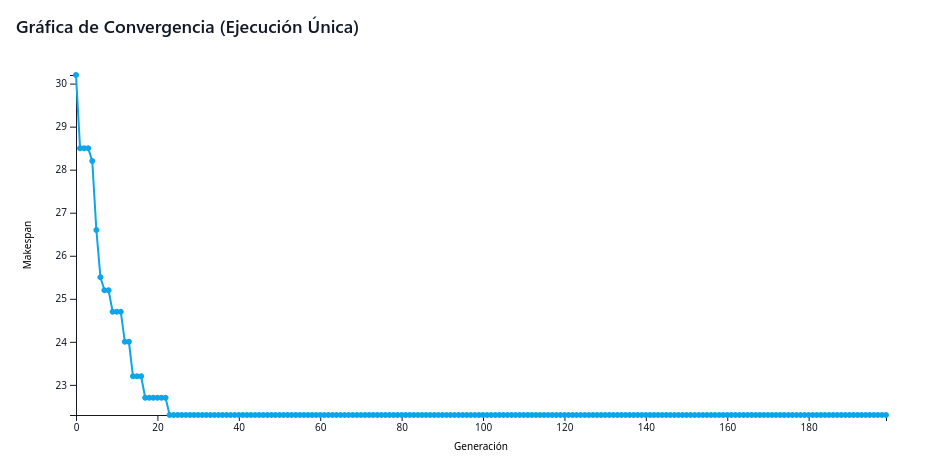
\includegraphics[width=0.9\textwidth]{assets/convergencia_ej_1.png}
    \caption{Gráfica de convergencia para el escenario 1.}
\end{figure}

\begin{figure}[H]
    \centering
    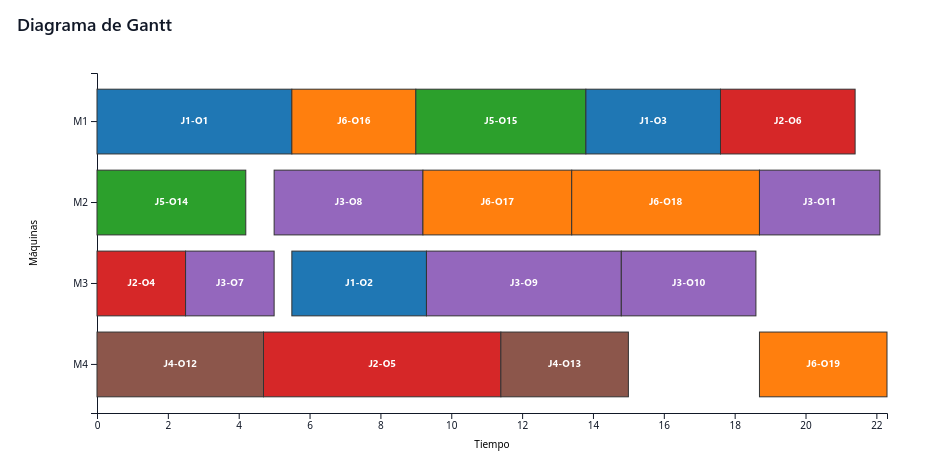
\includegraphics[width=0.9\textwidth]{assets/gantt_ej_1.png}
    \caption{Diagrama de Gantt para el escenario 1.}
\end{figure}

\clearpage
\subsection*{Escenario 2}
\addcontentsline{toc}{subsection}{Escenario 2}

\begin{figure}[H]
    \centering
    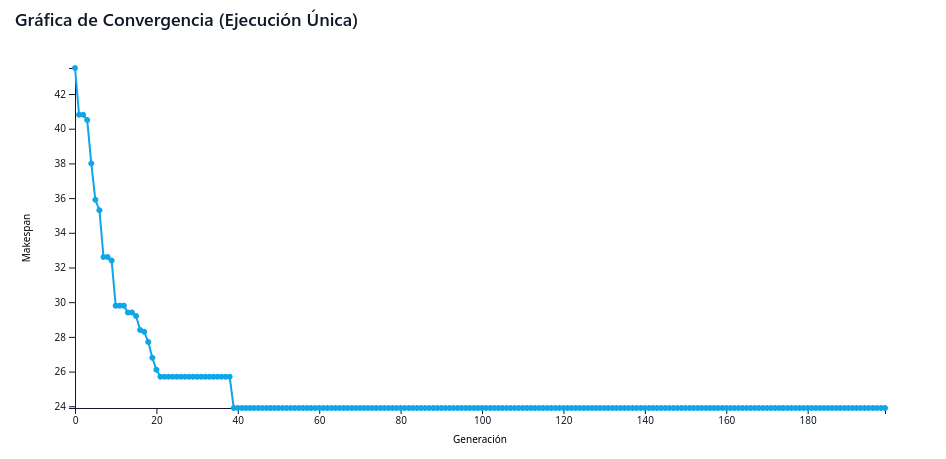
\includegraphics[width=0.9\textwidth]{assets/convergencia_ej_2.png}
    \caption{Gráfica de convergencia para el escenario 2.}
\end{figure}

\begin{figure}[H]
    \centering
    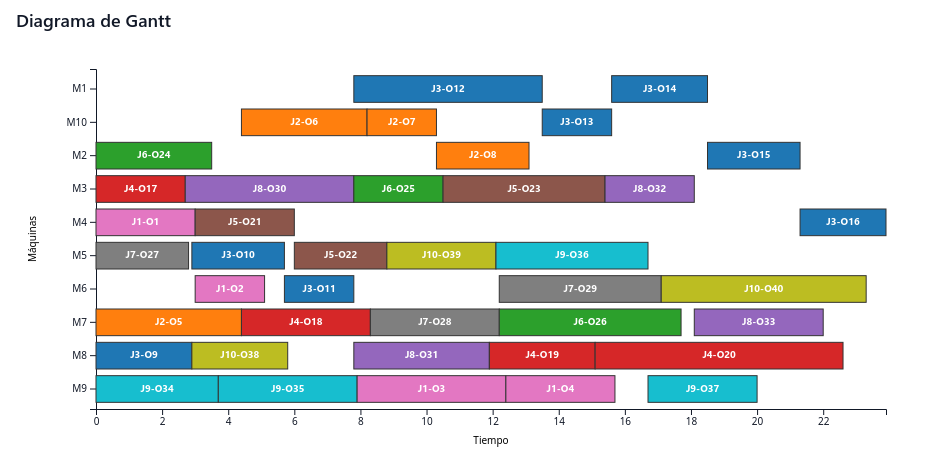
\includegraphics[width=0.9\textwidth]{assets/gantt_ej_2.png}
    \caption{Diagrama de Gantt para el escenario 2.}
\end{figure}

\clearpage
\subsection*{Escenario 3}
\addcontentsline{toc}{subsection}{Escenario 3}

\begin{figure}[H]
    \centering
    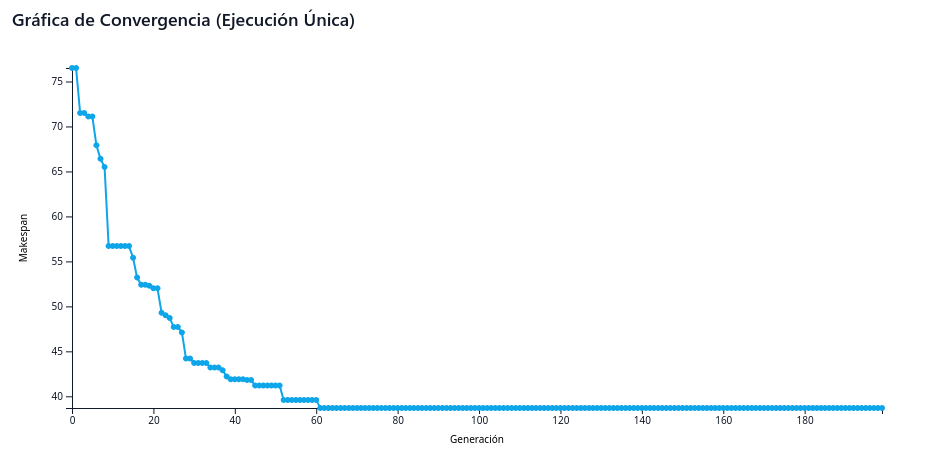
\includegraphics[width=0.9\textwidth]{assets/convergencia_ej_3.png}
    \caption{Gráfica de convergencia para el escenario 3.}
\end{figure}

\begin{figure}[H]
    \centering
    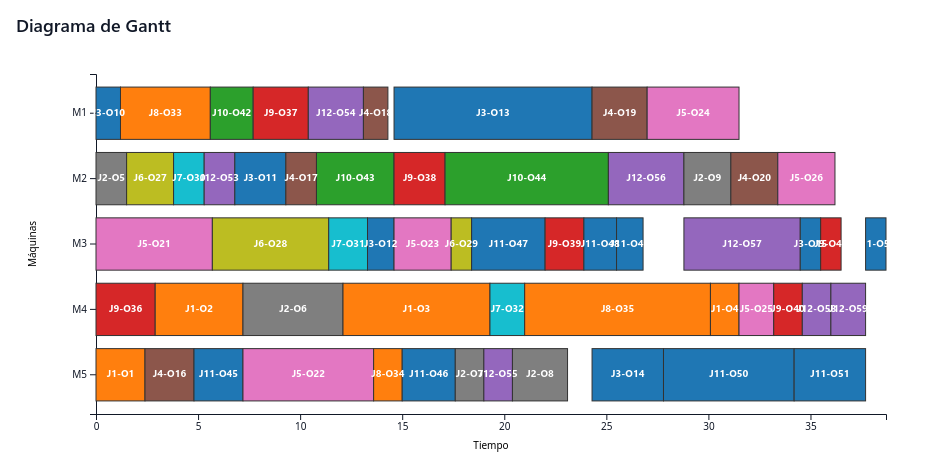
\includegraphics[width=0.9\textwidth]{assets/gantt_ej_3.png}
    \caption{Diagrama de Gantt para el escenario 3.}
\end{figure}

\bibliographystyle{IEEEtran}
\bibliography{references}

\end{document}
